\section{Statistica descrittiva}
\subsection{Vocabolario,Frequenze, frequenze relative, ...}
%%%%%%%%%%%%%%%%%%%%%%%%%%%%%%%%%%%%%%%%%%%%%%%%%%%%%%%%%%%%%%%%%%%%%%
%\subfile{../ch/BS-MPT-FP-rappel-fct-1-2}
\begin{questions}

\question
\exonly{
Indicare per ognuna delle seguenti variabili se sono quantitative (discrete o continue) o qualitative (nominali o ordinali). }


\begin{parts}
	\part \exonly{ Un negozio vende 3 tipi di bevande: bibite, tè e caffè  } \solonly{Qualitativa nominale }
	\part \exonly{ Il tempo di volo da Roma a Milano } \solonly{Quantitativa continua }
	\part \exonly{Numero di telefoni per nucleo famigliare  } \solonly{Quantitativa discreta }
	\part \exonly{Numero di telefonate per mese } \solonly{Quantitativa discreta }
	\part \exonly{Sesso (Uomo/Donna) } \solonly{Qualitativa nominale }
	\part \exonly{Possesso di uno smartphone (SI/NO) } \solonly{Qualitativa nominale }
	\part \exonly{ Titolo di studio  } \solonly{Qualitativa ordinale }
	\part \exonly{Grado di soddisfazione rispetto ad un’attività: Insufficiente, Discreto, Buono } \solonly{Qualitativa ordinale }
\end{parts}





%\end{questions}
%
%\section{Frequenze, frequenze relative, ...}
%
%\begin{questions}
\question

	

	
\begin{parts}
	\part \exonly{Completa la tabella }
	
		\begin{Tabular}[1.5]{|p{1cm}|p{2cm}|p{3cm}|p{3cm}|p{3cm}|p{3cm}|}
		\hline
		Classe & No allievi & \% degli allievi della classe rispetto al totale allievi & Promossi con 0 insufficienze & Promossi con 1 insufficienza & Promossi con 2  o più insufficienze \\ \hline \hline
		I° A   &   \solonly{21 }         & 33\%                                                     & 14                           &            \solonly{3 }                & 4                                   \\ \hline
		
		I° B   & 24         &                     \solonly{38\% }                                     & 12                           & 7                            & 5                                   \\ \hline
		
		I° C   &    \solonly{18 }        & 29\%                                                     & 8                            &             \solonly{6 }                 &                    \solonly{4 }                 \\ \hline\hline
		
		TOT. & 63         & 100\%                                                    &             \solonly{34 }                  & 16                           & 13    \\     \hline                         
	\end{Tabular}

\part \exonly{Calcola la percentuale dei promossi con insufficienze nella classe I B. } \solonly{50\% }
\part \exonly{Calcola la percentuale dei promossi senza insufficienze nelle tre classi messe assieme. } \solonly{54 \% }
\end{parts}

\question
\exonly{Da un collettivo di 20 individui si è rilevata la seguente distribuzione relativa ai caratteri “età”, “sesso”, “numero di automobili possedute in famiglia”: 


	\begin{Tabular}[1.5]{|l|l|l|l|l|l|l|l|l|l|l|l|l|l|l|l|l|l|l|l|l|}
		\hline
		Individuo   & 1  & 2  & 3  & 4  & 5  & 6  & 7  & 8  & 9  & 10 & 11 & 12 & 13 & 14 & 15 & 16 & 17 & 18 & 19 & 20 \\ \hline
		Età     & 35 & 37 & 59 & 54 & 44 & 38 & 62 & 71 & 56 & 60 & 33 & 46 & 41 & 53 & 38 & 55 & 50 & 63 & 35 & 51 \\ \hline
		Sesso   & M  & M  & F  & M  & F  & M  & F  & F  & M  & M  & M  & F  & F  & M  & F  & M  & M  & M  & F  & M  \\ \hline
		N. auto & 1  & 2  & 1  & 0  & 2  & 1  & 1  & 0  & 3  & 2  & 2  & 4  & 3  & 1  & 1  & 2  & 3  & 0  & 1  & 2  \\ \hline
	\end{Tabular}


}

\begin{parts}
	\part \exonly{Costruire la tabella delle distribuzioni di frequenza  per i caratteri “sesso” e “N. auto” }
	\solonly{
	\begin{tabular}{|l|l|}
		\hline
		Sesso & Freq. Assoluta \\ \hline
		F    & 8              \\ \hline
		M    & 12             \\ \hline
		TOT. & 20             \\ \hline
	\end{tabular}
\begin{tabular}{|l|l|}
	\hline
	No. Auto & Freq. Assoluta \\ \hline
	0        & 3             \\ \hline
	1        & 7              \\ \hline
	2        & 6             \\ \hline
	3        & 3             \\ \hline
	4        & 1             \\ \hline
	TOT.     & 20             \\ \hline
\end{tabular}


 }
	
	\part 
	
	\exonly{Considerare il carattere “età” suddiviso nelle seguenti classi: $[30;40[$ ,  $[40;50[$; $[50;60[$ ,  $[60+]$ , e costruire le corrispondenti distribuzioni di frequenza assolute, relative e percentuali. }
	
	\solonly{
	
\begin{Tabular}[1.5]{|l|l|l|l|}
	\hline
	Classe età  & Freq. Assoluta & Freq. Relativa & Percetuale \\ \hline
	{[}30;40{[} & 6              & 0.3            & 30\%       \\ \hline
	{[}40;50{[} & 3              & 0.15           & 15\%       \\ \hline
	{[}50;60{[} & 7              & 0.35           & 35\%       \\ \hline
	60+         & 4              & 0.2            & 20\%       \\ \hline
	TOT.        & 20             &                &            \\ \hline
\end{Tabular}

 }
\end{parts}

\exnewpage
\question
\exonly{Costruire le distribuzioni di frequenze relative e percentuali per ogni variabile
	considerata.
 }

\begin{Tabular}[1.5]{|l|l|l|l|}
	\hline
	Gruppo sanguigno & Frequenza assoluta & Frequenza relativa & Frequenza percentuale \\ \hline
	0                & 9                  & \solonly{0.45 }               & \solonly{45\%  }                 \\ \hline
	AB               & 3                  & \solonly{0.15 }               & \solonly{15\%  }                 \\ \hline
	A                & 3                  & \solonly{0.15 }               & \solonly{15\%  }                 \\ \hline
	B                & 5                  & \solonly{0.25  }              & \solonly{25\%  }                 \\ \hline
	TOTALE           & \solonly{20  }                &                    &                       \\ \hline
\end{Tabular}

\question
\exonly{La seguente tabella riporta i punteggi ottenute da una classe alla fine di un corso
	universitario.

\begin{Tabular}[1.5]{l|l|l|l|l|l|l|l|l|l|l|l|l|l|l}
%	\hline
	Nota (Max.30) & 18 & 19 & 20 & 21 & 22 & 23 & 24 & 25 & 26 & 27 & 28 & 29 & 30 & totale \\ \hline
	N. studenti   & 7  & 2  & 5  & 1  & 3  & 2  & 12 & 1  & 8  & 4  & 6  & 1  & 5  & 57     \\ %\hline
\end{Tabular}

 }

\begin{parts}
	\part \exonly{Calcolare la distribuzione delle frequenze cumulate relative avendo suddiviso il carattere nelle seguenti  classi: 
		$18-22$, $23-24$, $25-26$, $27-28$, $29-30$.
	 }
 
 \solonly{
 
\begin{Tabular}[1.5]{|l|l|l|l|l|}
\hline 
Punti & N. studenti & Freq. Rel. & Freq. Cum. Ass. & Freq. Cum. Rel. \\ \hline \hline
18-22 & 18          & 32\%       & 18              & 32\%            \\ \hline
23-24 & 14          & 25\%       & 32              & 56\%            \\ \hline
25-26 & 9           & 16\%       & 41              & 72\%            \\ \hline
27-28 & 10          & 18\%       & 51              & 89\%            \\ \hline
29-30 & 6           & 11\%       & 57              & 100\%           \\ \hline \hline
TOT.  & 57          &            &                 &                 \\ \hline 
\end{Tabular}
 }

\part \exonly{Cosa si può dire a proposito delle classi modali indicate? } \solonly{Più di metà della classe ha una nota inferiore a 24. }

\part \exonly{Quanti sono gli studenti che hanno ottenuto un voto inferiore o uguale a 26? } 
 \solonly{ Sono 41. Il 72\% della classe.}

\part \exonly{Quanti sono gli studenti che hanno ottenuto un voto non superiore a 24? }
\solonly{Sono 32. Il 56\% della classe. }

\part \exonly{Quanti studenti hanno ottenuto un voto superiore a 26? }
\solonly{$57-41=16$ studenti }
\end{parts}


\question
\exonly{Consideriamo il salario degli impiegati di una singola azienda. 

}

\begin{parts}
\part

\exonly{ Completare la tabella con frequenze cumulate, relative percentuali e relative cumulate.

\begin{Tabular}[1.5]{|c|c|c|c|c|}
\hline

Salario & Freq. Ass. & Freq. Ass. cumulata & Freq. Rel. & Freq. Rel. cumulata  \\ \hline \hline
[3500;4000[ & 8 &  &  &   \\ \hline
[4000;4500[ & 15 &  &  &    \\ \hline
[4500;5000[ & 21 &  &  &    \\ \hline
[5000;5500[ & 18 &  &  &    \\ \hline
  [5500;6000[ & \cellcolor[gray]{.8} 9 & \cellcolor[gray]{.8} & \cellcolor[gray]{.8} &  \cellcolor[gray]{.8}  \\ \hline
[6000;6500[ & 2 &  &  &    \\ \hline \hline
Totale &  &  &  &    \\ \hline

\end{Tabular}


}

\solonly{
\begin{Tabular}[1.5]{|c|c|c|c|c|}
 \hline
 Salario & Freq. Ass. & Freq. Ass. cumulata & Freq. Rel. & Freq. Rel. cumulata \\ \hline \hline
 [3500;4000[ & 8 & 8 & 11\% & 11\% \\ \hline
 [4000;4500[ & 15 & 23 & 21\% & 32\% \\ \hline
 [4500;5000[ & 21 & 44 & 29\% & 60\% \\ \hline
 [5000;5500[ & 18 & 62 & 25\% & 85\% \\ \hline
 [5500;6000[ & 9 & 71 & 12\% & 97\% \\ \hline
 [6000;6500[ & 2 & 73 & 3\% & 100\% \\ \hline \hline
 Totale & 73 &  &  &  \\ \hline
\end{Tabular}
}

\part

\exonly{Inserire ogni valore della riga grigia in una frase che parli di questa statistica.}

\solonly{
Il 12\% degli impiegati (9 impiegati) guadagnano tra i 5500 e i 6000 Fr. \\
Praticamente tutti gli impiegati (il 97\%, ovvero 71 impiegati) dell'azienda guadagna meno di 6000 Fr. \\


}
\end{parts}




\end{questions}


\exnewpage
\subsection{Rappresentazioni grafiche}
\begin{questions}
\question
\exonly{Nella tabella seguente sono riportate le risorse di un paese. Completare la tabella determinando l’ampiezza del settore circolare corrispondente e disegnare il diagramma circolare.

\begin{Tabular}[1.5]{|l|l|l|}
\hline

Attività & Percentuale & Ampiezza del settore \\ \hline
Industria & 45\% & \\ \hline
Agricoltura &30\%  & \\ \hline
Servizi & 15\% & \\ \hline
Altro &10\% &\\ \hline
\end{Tabular}
}

\solonly{
\begin{tikzpicture}
\pie{ 45/Industria, 30/Agricoltura, 15/Servizi, 10/Altro}
\end{tikzpicture}

}


\question
\exonly{
Il seguente grafico riporta la frequenza cumulata nella popolazione maschile. 

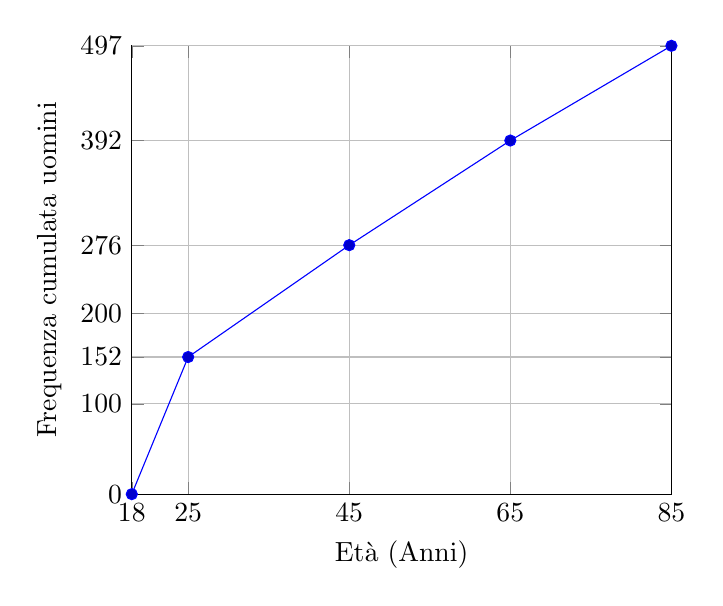
\begin{tikzpicture}
\begin{axis}
[ylabel=Frequenza cumulata uomini,
xlabel=Età (Anni),
enlargelimits=0,
ytick={0,100,200,500,600},
extra y ticks = {152,276,392,497},
ymajorgrids,
xmajorgrids,
minor y tick num=1,
yminorticks=true,
yminorgrids,
xtick={18,25,45,65,85}]
\addplot  coordinates
{ (18,0) (25,152) (45,276) (65,392) (85,497) };
\end{axis}

\end{tikzpicture}

}



\exonly{
Per le donne è data la tabella delle frequenze.

\begin{Tabular}[1.5]{|l|l|l|l|l|}
\hline

Donne &  [18;25[ &  [25;45[ &  [45;65[ &  [65;85[ \\ \hline
Frequenza & 68 & 136 & 105 & 94 \\ \hline

\end{Tabular}
}

\begin{parts}
\part
\exonly{Nel grafico cosa stanno ad indicare i valori 18, 25, 45, ecc.?}
\solonly{I bordi delle classi di età degli uomini della popolazione indagata.}
\part
\exonly{Nel grafico cosa sta ad indicare 152?}
\solonly{152 uomini hanno meno di 25 anni (tra i 18 e i25)}

\part
\exonly{Nel grafico cosa sta ad indicare 276?}
\solonly{276 uomini hanno meno di 45 anni.}

\part
\exonly{Costruire la tabella delle frequenze per gli uomini.}
\solonly{
\begin{Tabular}[1.5]{|l|l|l|l|l|}
\hline

Uomini &  [18;25[ &  [25;45[ &  [45;65[ &  [65;85[ \\ \hline
Frequenza & 152 & 124 & 116 & 105 \\ \hline

\end{Tabular}
}

\part
\exonly{Quante donne compongono la popolazione indagata?}
\solonly{403 donne}

\part
\exonly{In percentuale rispetto alla popolazione totale, quanti uomini compongono la popolazione indagata?}
\solonly{Circa il 55\% della popolazione totale.}

\part\label{ex:perc-uomini}
\exonly{Quanti uomini, in percentuale, rispetto a tutti gli uomini della popolazione hanno meno di 45 anni?}
\solonly{Circa il 56\% degli uomini.}

\part\label{ex:perc-donne}
\exonly{Quante donne, in percentuale, rispetto a tutte le donne della popolazione hanno meno di 45 anni?}
\solonly{Circa il 51 \% delle donne.}

\part\label{ex:perc-tot}
\exonly{Quanti uomini e donne, in percentuale, rispetto a tutta la popolazione hanno meno di 45 anni?}
\solonly{Circa il 53\% della popolazione totale.}

%\part
%\exonly{La media della risposta al punto (\ref{ex:perc-uomini}) e (\ref{ex:perc-donne}) è esattamente uguale al valore trovato al punto (\ref{ex:perc-tot}). Come mai?}
\end{parts}


\exnewpage
\question
\exonly{Il grafico riportato sotto illustra il numero di veicoli immatricolati nel cantone dal 1990 al 2010.
Quale messaggio viene veicolato da questo grafico? Ci sono degli errori? E se si quali?

\includegraphics[scale=0.6]{es-grafico-auto}


}
\solonly{Discussione in classe }


\question
\exonly{ 
I due grafici qui sotto rappresentano l’evoluzione del consumo di birra per abitante in Svizzera dal 1981 al 1984.
Quale delle due affermazioni è corretta? Quali elementi del grafico cercano di ingannare il lettore?

\begin{figure}[h!]
\centering
\begin{minipage}{.5\textwidth}
  \centering
  \begin{tikzpicture}
  \begin{axis}[
  AxisDefaults,
  ylabel style={},
  %TinyAxisLabels,
      axis y line=middle, 
      axis x line=bottom,
      xlabel={},
  	ylabel={Consumo [$L/\text{anno}$]},
  xmin=0,
  xmax=3,
  ymin=0,
  ymax=80,
  ytick distance=10,
  xtick={0,1,2,3},
  xticklabels={1981,1982 ,1983 , 1984}
  ]
  \plot[very thick] {-8*x/15+70.2};
  \end{axis}
  \end{tikzpicture}
  \captionof{figure}{Gli Svizzeri bevono sempre tanta birra!}
\end{minipage}%
\begin{minipage}{.5\textwidth}
  \centering
  \begin{tikzpicture}
  \begin{axis}[
  AxisDefaults,
  ylabel style={},
  %TinyAxisLabels,
      axis y line=middle, 
      axis x line=bottom,
      xlabel={},
  	ylabel={Consumo [$L/\text{anno}$]},
  xmin=0,
  xmax=3,
  ymin=68,
  ymax=71,
  ytick distance=0.5,
  xtick={0,1,2,3},
  xticklabels={1981,1982 ,1983 , 1984}
  ]
  \plot[very thick] {-8*x/15+70.2};
  \end{axis}
  \end{tikzpicture}
  \captionof{figure}{Gli Svizzeri bevono meno!}
  \label{fig:test2}
\end{minipage}
\end{figure}


}

\solonly{Discussione in classe }



\question
\exonly{ Data la  distribuzione di una variabile qualitativa nominale (vedi tabella) calcolare le frequenze relative e rappresentare graficamente la distribuzione così ottenuta mediante un grafico a nastri.

\begin{Tabular}[1.5]{|l|l|}
	\hline
	
	 & Freq. assolute cumulative \\ \hline
	A & 25 \\ \hline
	B & 75 \\ \hline
	C & 95 \\ \hline
	D & 100 \\ \hline
	
\end{Tabular}


 }

\solonly{
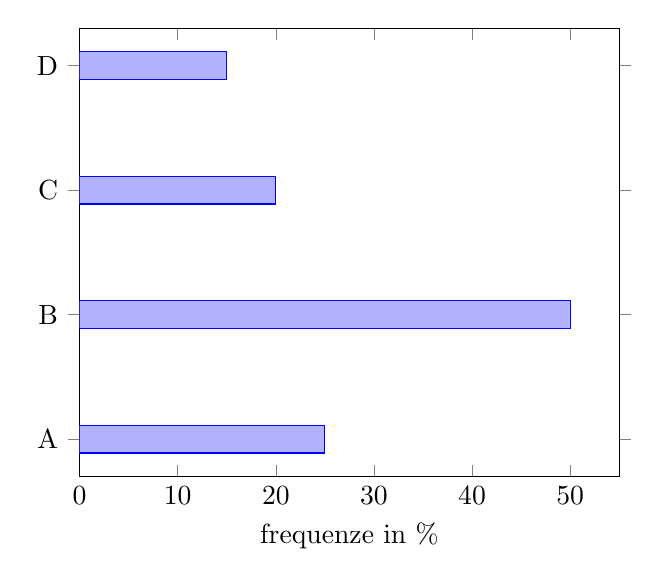
\begin{tikzpicture}
\begin{axis}[
xbar, xmin=0,
%width=12cm, height=3.5cm, enlarge y limits=-1.5,
xlabel={frequenze in \%},
symbolic y coords={A,B,C,D},
ytick=data,
%nodes near coords, nodes near coords align={horizontal},
]
\addplot coordinates {(25,A) (50,B) (20,C) (15,D)};
\end{axis}
\end{tikzpicture}
 }

\exnewpage
\question
\exonly{
Data la seguente distribuzione relativa ad una variabile continua X:

\begin{Tabular}[1.5]{|l|l|}
	\hline
	
	$X_j$ & Freq. relative  \\ \hline
	$[18;20[$ & 6\% \\ \hline
	$[20;25[$ & 10\% \\ \hline
	$[25;30[$ & 30\% \\ \hline
	$[30; 60[$ & 54\% \\ \hline
	
\end{Tabular}

Stimare la quota di individui con un valore della variabile: 
 }

\begin{parts}
	\part
	\exonly{inferiore a 19  }
	\solonly{3\% }
	\part
	\exonly{superiore a 22 }
	\solonly{90\% }
	\part
	\exonly{compreso fra 40 e 50 }
	\solonly{18\% }
\end{parts}


\question
\exonly{Associare i diagrammi delle frequenze cumulate con i rispettivi istogrammi. 

\includegraphics[scale=1]{istogrammma-diagramma_cum}
 }
\solonly{1-c, 2-b, 4-d, 5-a }

\question
\exonly{Data la seguente funzione di ripartizione: 
	
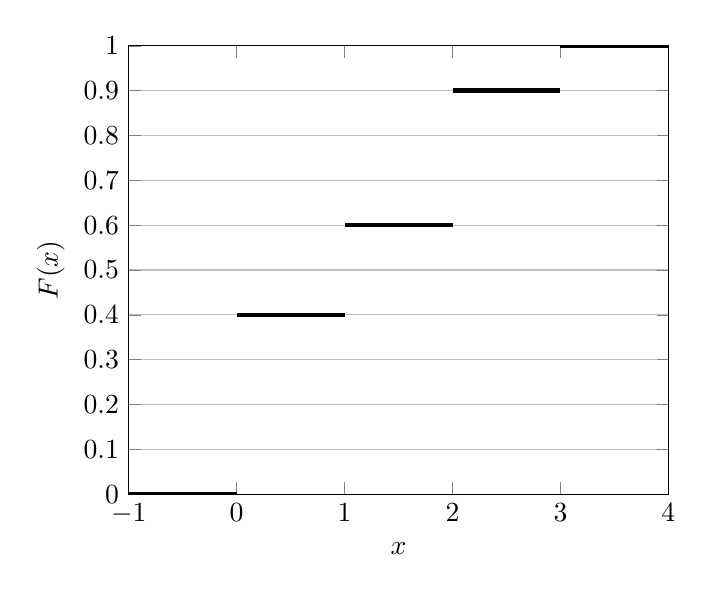
\begin{tikzpicture}
\pgfplotsset{every axis plot post/.append style={ultra thick,mark=none,black}}
\begin{axis}
[ylabel=$F(x)$,
xlabel=$x$,
enlargelimits=0,
ymajorgrids,
ytick distance={0.1},
ymax=1,
%extra y ticks={35,121,245},
xtick={-1,0,1,2,...,4}]
\addplot coordinates {(-1,0) (0,0)};
\addplot coordinates {(0,0.4) (1,0.4)};
\addplot coordinates {(1,0.6) (2,0.6)};
\addplot coordinates {(2,0.9) (3,0.9)};
\addplot coordinates {(3,1) (4,1)};
\end{axis}
\end{tikzpicture}
}

\begin{parts}
	\part 
	\exonly{ Quante sono le modalità? }
	\solonly{5 modalità (-1,0,1,2,3) }
	
	\part
	\exonly{$F(1.5) =$ }
	\solonly{ $F(1.5) = 0.6$   }
	
	\part
	\exonly{Definisci la funzione di ripartizione $F(x)$ }
	\solonly{$F(x) =\begin{cases} 0 & -1 \leq x <0 \\ 0.4 & 0 \leq x <1  \\ 0.6 & 1  \leq x < 2 \\ 0.9 & 2 \leq x <3 \\ 1 & 3 \leq x < 4\end{cases}$}

	\part
	\exonly{Ricostruire la tabella con le frequenze relative e le frequenze relative cumulate. }
	
\end{parts}

\end{questions}

\subsection{Indici di posizione centrale: moda, media, mediana}
\begin{questions}
	\question
	\exonly{Calcola la moda, la media e la mediana di questa distribuzione di frequenza.
	
\begin{Tabular}[1.5]{|l|l|l|l|l|l|l|}
	\hline
	
	$X_j$ & 1 & 2 & 4 & 5 & 6 & 7 \\ \hline
	$n_j$ & 2 & 3 & 5 & 1 & 1 & 2 \\ \hline
	

\end{Tabular} 

}
\solonly{Moda: 4, Media: 3.8 , Mediana: 4 }

\question
\exonly{
	Calcola la moda, la media e la mediana di questa distribuzione di frequenza.

\begin{Tabular}[1.5]{|l|l|l|l|l|l|l|}
	\hline
	
	$X_j$ & 2 & 3 & 4 & 5 & 6 & 7 \\ \hline
	$n_j$ & 3 & 4 & 1 & 5 & 5 & 6 \\ \hline
	
\end{Tabular}
 }
\solonly{Moda: 7, Media: 5 , Mediana: 5 }

\question
\exonly{In un quartiere viene recensito il numero di piani di ogni stabile.

\begin{tabular}{|C{3cm}|C{3cm}|} \hline 
	Numero \newline di piani & Freq. assoluta  \\ \hline\hline 
	1 & 10  \\ \hline 
	2 & 8   \\ \hline 
	3 & 14  \\ \hline 
	4 & 18   \\ \hline 
	5 & 15   \\ \hline 
	6 & 9   \\ \hline \hline
	\textbf{Totale} &    \\ \hline 
\end{tabular}

 }

\begin{parts}
	\part
	\exonly{Calcolare la media di piani degli stabili recensiti }
	\solonly{3.64 piani per stabile }
	\part
	\exonly{Calcolare la media di piani se ai dati iniziali aggiungiamo 3 immobili di 16 piani }
	\solonly{4.12 piani per stabile }
	\part
	\exonly{ Calcolare la media di piani se ai dati iniziali aggiungiamo 10 case  di 1 piano  }
	\solonly{3.32 piani per stabile }
	\part
	\exonly{Calcolare la media di piani se, sempre partendo dai dati iniziali, alzassimo 8 stabili di 1 piano. }
	\solonly{3.74 piani per stabile }
\end{parts}

\question
\exonly{ Determinare le tre misure di tendenza centrale di questa statistica che concerne il numero di impiegati di alcune piccole imprese.

\begin{Tabular}[1.5]{|C{3cm}|C{3cm}|C{3cm}|C{3cm}|} \hline 
	Numero di impiegati & Freq. assoluta &  &  \\ \hline\hline 
	1 & 22 &  &  \\ \hline 
	2 & 41 &  &  \\ \hline 
	3 & 55 &  &  \\ \hline 
	4 & 86 &  &  \\ \hline 
	5 & 108 &  &  \\ \hline 
	6 & 75 &  &  \\ \hline 
	7 & 42 &  &  \\ \hline 
	8 & 25 &  &  \\ \hline \hline
	\textbf{TOT} &  &  &  \\ \hline 
\end{Tabular}
 }
\solonly{Moda 5 , Media $4.62$ , Mediana $5$ }

\question
\exonly{Determinare le tre misure di tendenza centrale di questa statistica che concerne la superficie degli appartamenti abitativi di un quartiere.

\begin{Tabular}[1.5]{|C{3cm}|C{3cm}|C{3cm}|C{3cm}|C{3cm}|} \hline
	Superficie (in m${}^{2}$) & Freq. assoluta &  &  &  \\ \hline\hline 
	[0;20[ & 15 &  &  &  \\ \hline 
	[20;40[ & 18 &  &  &  \\ \hline 
	[40;60[ & 28 &  &  &  \\ \hline 
	[60;80[ & 51 &  &  &  \\ \hline 
	[80;100[ & 32 &  &  &  \\ \hline 
	[100;120[ & 19 &  &  &  \\ \hline \hline
	\textbf{TOT.} &  &  &  &  \\ \hline 
\end{Tabular}

 }
\solonly{Moda $[60;80[$ , Media $65.21$ , Mediana $74.64$ }
\end{questions}

\exnewpage

\subsection{Misure di dispersione: quartili, scarto quadratico medio}

\begin{questions}
		\question
	\exonly{
		Associare gli istogrammi ai boxplot corrispondenti.
		
		\includegraphics[scale=0.6]{istogrammi-boxplot} }
	\exonly{Discussione in classe }
	\question
	\exonly{
		Il servizio clienti di una grande ditta registra il numero di mail ai quali i suoi impiegati hanno risposto in un ora. I risultati sono sintetizzati nel boxplot qui sotto.
		
		\begin{tikzpicture}
		\begin{axis}
		[
		height=3cm,
		width=9cm,
		hide y axis,
		axis x line*=bottom,
		xtick distance=1,
		]
		
		\addplot+[
		boxplot prepared={
			median=8,
			upper quartile=14,
			lower quartile=5,
			upper whisker=18,
			lower whisker=2
		},
		] coordinates {};
		\end{axis}
		\end{tikzpicture}
	}
	
	\begin{parts}
		\part
		\exonly{Determinare i tre quartili della statistica e lo scarto interquartile. Interpretare i dati. }
		\solonly{$Q_1=5$ , $Q_2=8$ , $Q_3=14$ , scarto: $9$ }
		
		\part
		\exonly{ L'impiegato che ha risposto al minor numero di mail quanti ne ha trattati? E quello che ne ha trattai il maggior numero?  }
		\solonly{Minimo: 2, Massimo : 18 }
		
		\part
		\exonly{Che percentuale degli impiegati ha trattato 8 mail o più? }
		\solonly{50\% }
		
		\part
		\exonly{Che percentuale degli impiegati ha trattato tra i 5 e 14 mail? }
		\solonly{50\% }
		
		\part
		\exonly{Il quarto degli impiegati che ha risposto a meno casi quanti ne ha trattati ? }
		\solonly{Meno di 5 }
	\end{parts}

\question
\exonly{
	Ecco i risultati di 24 allievi per un esame (numero di punti massimi 100).

\begin{tabular}{llllllll}
	78 & 79 & 77 & 59 & 57 & 65 & 65 & 67 \\ 
	68 & 67 & 59 & 54 & 64 & 68 & 72 & 74 \\ 
	72 & 72 & 76 & 77 & 76 & 74 & 77 & 76 \\ 
\end{tabular}

 }

\begin{parts}
	\part
	\exonly{Determinare la mediana e i quartili di questa serie. }
	\solonly{Mediana: 72, $Q_1=65$, $Q_3=76$ }
	\part
	\exonly{Disegnare il boxplot }
	\solonly{
		\begin{tikzpicture}
	\begin{axis}
	[
	height=3cm,
	width=9cm,
	hide y axis,
	axis x line*=bottom,
	xtick distance=2,
	]
	
	\addplot+[
	boxplot prepared={
		median=72,
		upper quartile=76,
		lower quartile=65,
		upper whisker=79,
		lower whisker=54
	},
	] coordinates {};
	\end{axis}
	\end{tikzpicture}
 }

\part
\exonly{
Si possono comparare i risultati di questa classe con quelli di un'altra classe.

 Della seconda classe si sa che: le due note più basse sono 47 e 55 , la nota massima è 85, la mediana 70, Q1=67 e Q3=76. 
 
 Tracciare sullo stesso grafico anche questo boxplot e comparare le due classi.
 }

\solonly{
	\begin{tikzpicture}
\begin{axis}
[
height=3cm,
width=9cm,
hide y axis,
axis x line*=bottom,
xtick distance=2,
]

\addplot+[
boxplot prepared={
	median=72,
	upper quartile=76,
	lower quartile=65,
	upper whisker=79,
	lower whisker=54
},
] coordinates {};
\addplot+[
boxplot prepared={
	median=70,
	upper quartile=76,
	lower quartile=67,
	upper whisker=85,
	lower whisker=55
},
] coordinates {(0,47)};
\end{axis}
\end{tikzpicture}

 }
\end{parts}

\question
\exonly{
	La rappresentazione grafica seguente raffigura l'evoluzione del tasso di mortalità infantile (mortalità infantile per 1000 nascite in vita) dal 1901 al 1975 in Svizzera (dati dei 25 Cantoni).
	
	\includegraphics[scale=0.8]{box-plot-nascite}
	
Come interpretare le informazioni seguenti :
\begin{parts}
	\part I box sono sempre più piccoli 
	\part I box sono sempre più in basso
	\part Nel 1921 il baffo superiore è molto più grande di quello inferiore
	\part  In quale periodo la maggior parte dei cantoni aveva un tasso di mortalità  inferiore alla mediana? 
	\part I dati sono raggruppati su periodi di 5 anni e non di un anno? 
	\part Perché 25 cantoni e non 26? 
\end{parts} 
}

\solonly{Discussione in classe }
	
	\question
	
\exonly{Calcola media aritmetica, moda, mediana e scarto quadratico medio della seguente distribuzione di frequenza. 

\begin{Tabular}{|l|l|l|l|l|l|}
	\hline
	
	$X_j$ & 1 & 3 & 4 & 5 & 11 \\ \hline
	$n_j$ & 1 & 3 & 1 & 4 & 1 \\ \hline
	
\end{Tabular}
}

\solonly{Media: $\overline{x}=4.5$ e $\sigma=2.5$ , Moda: 5, Mediana: $\tilde{x}=4.5$}

 	\question
 	\exonly{
 	Calcola media aritmetica, moda, mediana e scarto quadratico medio della seguente distribuzione di frequenza. 
 

	\begin{Tabular}[1.5]{|l|l|l|l|l|}
		\hline
		
		$X_j$ & 1,4 & 2,4 & 3,4 & 4,4 \\ \hline
		$n_j$ & 1 & 1 & 1 & 4 \\ \hline
		
	\end{Tabular}
	 }
 	\solonly{Media: $\overline{x}=3.54$ e $\sigma=1.13$ , Moda: 4.4, Mediana: $\tilde{x}=4.4$}
 	
 	\exnewpage
 	\question
 	\exonly{
 	Sapendo che la distribuzione di frequenza 
 	
 	\begin{Tabular}[1.5]{|l|l|l|l|l|}
 		\hline
 		
 		$X_j$ & 5 & 10 & 15 & 20 \\ \hline
 		$n_j$ & \cellcolor[gray]{.9} $n_1$ & 3 & 1 & 1 \\ \hline
 		
 	\end{Tabular}

	ha media aritmetica $\overline{x}=9$, ricostruisci la frequenza mancante.
		 }
	 \solonly{$n_1=5$ }
 	
 	
	\question
	\exonly{Nell'ambito di un controllo di qualità (scegliendo un campione di lotto prodotti) si é notato il numero di pezzi difettati di ogni lotto esaminato.
	
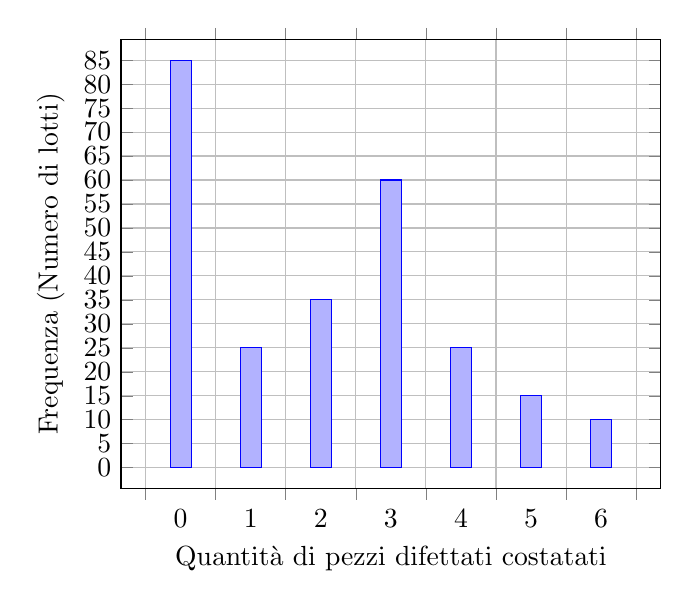
\begin{tikzpicture}
\begin{axis}[
xlabel = Quantità di pezzi difettati costatati,
xtick={1,...,7},
ytick={0,5,10,...,90},
grid=major,
%minor y tick num=1,
%x tick label style={rotate=45,anchor=east},
ylabel=Frequenza (Numero di lotti),
enlargelimits=0.05,
%legend style={at={(0.5,-0.15)}, anchor=north,legend columns=-1},
ybar interval=0.3,
%xticklabel shift={.3cm},
%xticklabel=[\pgfmathprintnumber\tick;\pgfmathprintnumber\nexttick [
]
\addplot coordinates
{(0,85) (1,25) (2,35) (3,60) (4,25) (5,15) (6,10) (7,0)};
\end{axis}
\end{tikzpicture}

 }


\exonly{Calcolare la media e lo scarto quadratico medio di pezzi difettati per lotto. Se siamo disposto a tollerare un massimo di 2 pezzi difettosi per lotto acquisteremmo da questo fabbricante? E se ne tollerassimo 3? Oppure 4?  }

\solonly{ $\bar{x}=2$ $\sigma=1.8$. Quindi maggioranza dei dati tra $[0;3]$.
	
	In generale avremo tra gli 0 i 3 pezzi difettosi in un lotto, quindi non acquisteremmo se tolleriamo al massimo 2 pezzi difettosi (molto spesso ce ne sono 3). Potremmo acquistare se ne tolleriamo 3 ma nel 15\% ca. dei casi potremmo averne 4. Se ne tollerassimo 4 acquisteremmo perché solo nel 2.5\% ca. dei casi i pezzi difettati saranno più di 4}


\question
\exonly{Determinare la media e lo scarto quadratico medio di questa statistica che si interessa alla durata delle telefonate di una classe della vostra scuola in una settimana 

\begin{Tabular}[1.5]{|C{2cm}|C{2cm}|C{2cm}|C{2cm}|C{2cm}|C{2cm}|} \hline 
	Durata della telefonata \newline (secondi) & Frequenza \newline assoluta  &  &  &    & \\ \hline \hline 
	[0;30[ & 45 &  &  &  &  \\ \hline 
	[30;60[ & 48 &  &  &  &  \\ \hline 
	[60;90[ & 77 &  &  &  &  \\ \hline 
	[90;120[ & 124 &  &  &  &  \\ \hline 
	[120;150[ & 88 &  &  &  &  \\ \hline 
	[150;180[ & 64 &  &  &  &  \\ \hline \hline 
	\textbf{TOT.} & 446 &  &  &  &  \\ \hline 
\end{Tabular}

}
\solonly{$\bar{x}= 98.81$ e $ \sigma=44.9$}

% 	\question
%\exonly{
%	Sapendo che la distribuzione di frequenza 
%	
%	\begin{Tabular}[1.5]{|l|l|l|l|l|}
%		\hline
%		
%		$X_j$ & 1 & 1.5 & 2 & 2.5 \\ \hline
%		$n_j$ & 4 & 1 & 2 & \cellcolor[gray]{.9} $n_4$ \\ \hline
%		
%	\end{Tabular}
%	
%	ha varianza $\sigma ^2=0.41$, ricostruisci la frequenza mancante.
%}
%\solonly{$n_4=$ }
\end{questions}



%\subsection{Esercizi ricapitolativi}